% \documentclass[notes=yes]{beamer}
\documentclass[12pt]{beamer}
% \usetheme{Warsaw}
\usepackage{amsmath}
\usepackage{graphicx}
% \usepackage{pgfpages}
\usepackage{siunitx}

\usepackage[utf8]{inputenc}
\usepackage[english]{babel}
 
\usepackage[
backend=biber,
style=alphabetic,
citestyle=phys
]{biblatex}

% \setbeameroption{show notes on second screen=right}
% \setbeamertemplate{note page}{\pagecolor{yellow!5}\insertnote}\usepackage{palatino}

\addbibresource{sources.bib}

\usecolortheme{dove}
\usefonttheme[onlymath]{serif}
% \usepackage{

\title{Building a LEGO Watt Balance}
\author{Michael Laraia, Jack Hirschi}
\institute{University of Minnesota}
\date{May 6, 2019}

\begin{document}
\begin{frame}
\titlepage
\end{frame}

\begin{frame}{SI Units}
    \only<1>{\begin{figure}
        \centering
        \includegraphics[width=0.5\linewidth]{figs/si_units_old.png}
        \caption{\cite{wiki_si_old}}
    \end{figure}}
    
    \only<2>{\begin{figure}
        \centering
        \includegraphics[width=0.5\linewidth]{figs/si_old_2.png}
        \caption{\cite{wiki_si_old}}
    \end{figure}}
\end{frame}

\note[itemize]{
    \item SI system is a collection of units defined based on some known constants
    \item Originally the units were defined based on some arbitrary constant
    \item Today we are pushing to redefine the units in terms of fundamental constants of the Universe
    \begin{itemize}
        \item meters in terms of the speed of light
        \item seconds in terms of the periodic decay of cesium atom
    \end{itemize}
    \item The kilogram is one of the last remaining units to be redefined in this way
    }

\begin{frame}{International Prototype Kilogram}
    \begin{figure}
        \centering
        \includegraphics[width=0.5\linewidth]{figs/ipk.png}
        \caption{\cite{ipk}}
    \end{figure}
    
\end{frame}

\note[itemize]{
    \item Forged in 1889 out of platinum-iridium alloy
    \item Only mass in the universe with no uncertainty in its mass
    \begin{itemize}
        \item $m=\si{1kg} \pm 0$
    \end{itemize}
    \item Problematic
}
\begin{frame}
    
    \begin{figure}
        \centering
        \includegraphics[width=0.8\linewidth]{figs/ipk_mass_drift.png}
        \caption{Change in mass of official IPK copies over time \cite{ipk_drift}.}
    \end{figure}
    
    \only<2>{
    \begin{itemize}
        \item The mass of the IPK is not guaranteed to be stable over time
        \item The SI system should not rely on an unstable reference definition
    \end{itemize}}
    
\end{frame}

\note[itemize]{
    \item There are multiple identical copies of the IPK
    \item The mass of these copies compared to the IPK have been drifting over time
    \begin{itemize}
        \item Corrosion
        \item Dust sticking to the surface
    \end{itemize}
    \item The official copies have been gaining mass over time relative to IPK
    \item The mass of the ipk is not guaranteed to be stable over time
}


\begin{frame}{New SI}
    \begin{figure}
        \centering
        \includegraphics[width=0.5\linewidth]{figs/si_units.png}
        \caption{\cite{wiki_si}}
    \end{figure}
\end{frame}

\note[itemize]{
    \item A few methods have been proposed to fix the kilogram to a universal constant
    \item One method is to use a Watt balance to fix the kilogram to Planck's constant.
}

\begin{frame}{Watt Balance}
    % \begin{figure}
    %     \centering
    %     \includegraphics[width=0.75\linewidth]{figs/paper_diagram.jpg}
    %     \caption{\cite{Chao2015}}
    % \end{figure}
    \begin{figure}
        \centering
        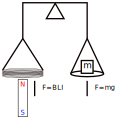
\includegraphics[width=0.6\linewidth]{figs/watt-balance-concept.png}
        % \caption{}
    \end{figure}
\end{frame}

\note[itemize]{
    \item Balance electrical power with mechanical power
}

\begin{frame}{Faraday's Law}
    \begin{figure}
        \centering
        \includegraphics[width=0.8\linewidth]{figs/faraday.png}
        % \caption{}
        \label{fig:faraday}
    \end{figure}
    
    \pause
    \begin{align*}
    \mathcal{E}= -N\frac{d\Phi_B}{dt}
    \end{align*}

\end{frame}

\begin{frame}{Lorentz Forces}
    \only<1>{\begin{align*}
        \vec{F} = q\vec{E} + q\vec{v}\times \vec{B}
    \end{align*}}
    \only<2>{\begin{align*}
        \vec{F} = q\vec{v}\times \vec{B}
    \end{align*}}
    \only<3>{\begin{align*}
        \vec{F} = \vec{I}L\times \vec{B}
    \end{align*}}
    \only<4>{\begin{align*}
        F = (\Phi_B L) I
    \end{align*}}
\end{frame}

\begin{frame}{Force Mode}
    \begin{figure}
        \centering
        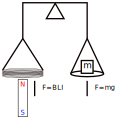
\includegraphics[width=0.6\linewidth]{figs/watt-balance-concept.png}
        % \caption{}
    \end{figure}
    
    \begin{align*}
        \Phi_B LI=mg
    \end{align*}
    
\end{frame}

\begin{frame}{Velocity Mode}
    \begin{figure}
        \centering
        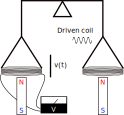
\includegraphics[width=0.6\linewidth]{figs/watt-balance-concept-vmode.png}
        % \caption{}
    \end{figure}
    
    \begin{align*}
        V=\Phi_B Lv
    \end{align*}
\end{frame}

\begin{frame}{Watt Balance Mechanics}
    % Might decide to nix the derivation part of it, and somehow incorporate
    % it into the discussion for the above images
\begin{align*}
    V &=(\Phi_B L)v \\
    mg &= (\Phi_B L)I \\
    \only<2>{(\Phi_B L)_v &= \frac{V}{v}\quad (\Phi_B L)_F = \frac{mg}{I} \\}
    \only<3>{m &= \frac{VI}{gv}}
\end{align*}

\end{frame}

\begin{frame}{Watt Balance}
    \begin{figure}
        \centering
        \includegraphics[width=0.75\linewidth]{figs/paper_diagram.jpg}
        \caption{\cite{Chao2015}}
    \end{figure}
\end{frame}
    
    

%   \begin{frame}
%     \frametitle{This is the first slide}
%     %Content goes here
%   \end{frame}
%   \begin{frame}
%     \frametitle{This is the second slide}
%     \framesubtitle{A bit more information about this}
%     %More content goes here
%   \end{frame}
% etc
\begin{frame}[allowframebreaks]{References}
    % \bibliographystyle{plainnat}
    \printbibliography
\end{frame}
\end{document}